%                                                       -*- coding: utf-8 -*-
% SI3: Projet Serveur Web
%
%%           Author: Erick Gallesio [eg@unice.fr]
%    Creation date:  2-Jun-2013 16:20 (eg)
% Last file update:  2-Jun-2013 20:31 (eg)

\documentclass[10pt,a4paper]{article}
\usepackage[utf8]{inputenc}
\usepackage[pdftex]{graphicx}
\usepackage{a4wide}
\usepackage[colorlinks=true,urlcolor=blue]{hyperref}
\usepackage{alltt}
\usepackage{fancyhdr}
\pagestyle{fancy}

%\input{exemples/pygments.tex}

\begin{document}

\newcommand{\promo}{2012-2013}

\thispagestyle{empty}
% Header
\lhead{}
\chead{}
\rhead{}
\renewcommand{\headrulewidth}{0pt}
%Footer
\lfoot{\footnotesize\sc SI3 - \promo}
\cfoot{\thepage{}}
\rfoot{\footnotesize\sc Projet}
\renewcommand{\footrulewidth}{0.4pt}


% ----------------------------------------------------------------------


\noindent

\includegraphics[width=4cm]{Ressources/pns.png}

\noindent
{\sc SI3 / \promo}\\
{\sc\small Erick Gallesio}
\vskip1cm

\parindent0pt

\begin{center}
{\huge  Projet SI3}\\[4mm]
{\bf \emph{Un serveur Web modulaire}}
\end{center}

Le but de ce projet est d'écrire un serveur Web modulaire en C. Les
principales caractéristiques de ce serveur, que nous appelerons
\texttt{polyweb}, sont détaillées ci-dessous. Toutefois, avant de
commencer à décrire le serveur à proprement parler, un certain nombre
de principes sur les réseaux et le protocole HTTP vont être
présentés. Ces principes sont ultra simplifiés pour rester
compréhensibles par tout un chacun.

Les fichiers qui vous sont distribués permettent de construire et donc
d'exécuter \texttt{polyweb}. Par contre la plupart des codes sources
de ce programme ne vous sont pas livrés. Votre travail va consister à
réécrire les différents composants du serveur et à reconstruire
les sources de ces  composants. Ainsi, vous aurez toujours un
programme qui fonctionne en substituant petit à petit les composants
qui vous ont été distribués, par ceux que vous avez réécrits.

Parmi les fichiers sources qui vous sont distribués, il y a un certain
nombre de \emph{headers} (des ``.h'') qui définissent l'interface des
composants qui vous sont donnés. Ces fichiers sont des
\textbf{contrats} et ne \textbf{doivent pas} être modifiés. Les
modules que vous remplacerez doivent être \textbf{compatibles} avec
l'interface décrite dans le \emph{header} correspondant.



%%%%%%%%%%%%%%%%%%%%%%%%%%%%%%%%%%%%%%%%%%%%%%%%%%%%%%%%%%%%%%%%%%%%%%
\section*{Réseaux: principes de base}

Lorsqu'on veut travailler avec une machine distante (pour copier des
fichiers, se connecter, parcourir une page web, jouer, lire son mail,
...), il faut en fait connaître 3 informations:
\begin{itemize}
\item le nom de la machine sur laquelle on veut se connecter (on
  l'appellera le serveur).
\item le protocole que l'on va utiliser: HTTP pour le Web, IMAP ou POP3
  pour le mail, SSH pour se connecter (ou exécuter une commande) sur la
  machine distante, ...
\item le numéro du port que l'on va utiliser. La plupart du temps, le
  numéro de port est implicite (e.g. 80 pour faire de l'HTTP, 143 pour
  faire de l'IMAP, 993 si l'IMAP est sécurisé, 22 pour SSH, ...). Rien
  n'empêche de faire de l'HTTP sur un autre port que 80 ou du SSH sur
  le port 22. Nous verrons cela plus tard.
\end{itemize}

Bref, quand vous entrez par exemple sur votre navigateur l'adresse
\url{http://wwww.google.fr} pour vous connecter à Google, le
navigateur établit en fait une connexion sur le serveur nommé
\texttt{www.google.fr} en utilisant le protocole HTTP. Comme vous
n'avez rien dit sur le port utilisé, le navigateur utilisera le port
par défaut (i.e. le port 80).  En fait, vous auriez pu entrer l'URL
\url{http://wwww.google.fr:80} pour expliciter le port de
connexion.


\section*{Réseau en C}

Il existe de nombreuses primitives pour faire du réseau en C.
Malheureusement celles-ci, sont d'assez bas niveau. Il ne sera pas
nécessaire de comprendre comment les choses marchent dans le détail.
Les fichiers \texttt{src/network.c} et \texttt{include/network.h}
permettent des s'abstraire des détails sordides. Trois primitives sont
définies:
\begin{itemize}
\item \texttt{create\_server}: permet de créer un serveur en
  attente sur le port qui a été passé en paramètre.
\item \texttt{accept\_connection}: permet d'attendre qu'un client
  arrive.  Lorsqu'un client se présente, la fonction remplit une
  structure de données de type \texttt{struct client\_info} qui contient
  des informations sur le client (son numéro IP et le nom de sa
  machine) ainsi qu'un descripteur de fichier permettant de discuter
  avec le client. Ce descripteur de fichier est ouvert en lecture et
  en écriture. Comme le protocole HTTP, utilisé par le web, est basé
  sur la notion de ligne, cette structure propose aussi deux champs
  \texttt{fin} et \texttt{fout} qui contiennent des \texttt{FILE *}
  permettant la lecture et l'écriture va et vers le client en mode
  ``bufferisé''.
\item \texttt{shutdown\_connection} permet de fermer la connexion vers
  le client.
\end{itemize}

Deux exemples de serveurs sont donné dans le répertoire \texttt{tests}
(\texttt{simple-server} et \texttt{multi-server}):
\begin{itemize}
\item \texttt{simple-server.c} est un serveur simple pour illustrer
  comment se servir du fichier \texttt{network.c}. Ce programme lit
  une ligne de son client et lui renvoie cette ligne convertie en
  majuscules.
\item \texttt{multi-server.c} est une petite modification du serveur
  précédent. Cette version lance un nouveau processus à chaque fois
  que l'on a un nouveau client. On peut donc avoir plusieurs clients
  simultanés. Pour chaque clien, les caractères saisis sont mis en
  majuscules (et seulement ceux qui sont saisis dans le client).  Dans
  la fenêtre du serveur, on voit par contre toutes les lignes lues,
  quelque soit le client où elles on été saisies.
\end{itemize}


Pour travailler avec ce serveur (c'est à dire pour être un client de ce serveur), il suffit de lancer le programme dans
un terminal et de lancer la commande suivante\footnote{la commande
  \texttt{netcat} (aussi appelée \texttt{nc}) est un une sorte de
  \texttt{cat} sur le réseau (d'où son nom ;-).} d'un \textbf{autre}
terminal\footnote{Par convention, la machine locale est toujours
  accessible par le nom \texttt{localhost}.}:
\begin{verbatim}
    $ netcat localhost 1234
\end{verbatim}
puisque le server tourne sur le port 1234 par défaut.

\section*{HTTP: principes de base}

Le protocole HTTP est un protocole relativement simple utilisé pour
``servir'' des pages Web. Nous n'allons pas voir ce protocole en
détails ici et nous nous bornerons aux méthodes GET et POST qui sont les plus
utilisées (la plupart des \emph{vrais} serveurs Web n'implémentent en
général que trois ou quatre des sept méthodes définies par le protocole HTTP).


Une requête HTML est formée d'une suite de lignes dont la dernière
est une ligne vide. La première ligne contient la commande à exécuter
(pour accéder à une page, on utilise la requête GET). Ensuite, se
trouvent des lignes précisant la requête (le type de fichier que l'on
sait traiter, les langues connues, le nom de navigateur, ...). Voici
un exemple de requête pour accéder à la page principale du site
\texttt{http://www.polytech.unice.fr}
\begin{alltt}
    GET / HTTP/1.0
    Host: www.polytech.unice.fr
    User-agent: Fait a la main v0.0
              \textcolor{red}{<== ligne vide: on a fini de discuter}
\end{alltt}

Ici , on déclare que l'on veut accéder la page principale (elle
s'appelle ``/'') et que l'on utilise la version 1.0 du protocole
HTTP.  La ligne \texttt{Host:} indique que l'on veut se connecter sur le
serveur \texttt{www.polytech.unice.fr} (ce qui est déjà le cas, mais
un serveur Web peut servir plusieurs domaines) et que notre browser Web
s'appelle ``Fait a la main v0.0''). Les deux dernières lignes ne sont,
en principe, pas obligatoires, mais certains serveurs Web les
exigent; il est donc plus prudent de les mettre systématiquement.

Essayons maintenant une connexion sur le serveur Web de l'école. Pour
cela, nous allons encore utiliser la commande \texttt{netcat}. Un
exemple de session est donné ci-dessous.

\begin{alltt}
    balico\$ netcat www.polytech.unice.fr 80
    GET / HTTP/1.0
    Host: www.polytech.unice.fr
    User-agent: Fait a la main v0.0
                            \textcolor{red}{<= ligne vide = on a fini notre requête}
    HTTP/1.1 200 OK         \textcolor{red}{<= À partir de là, entête de la réponse}
    Date: Wed, 02 Jan 2008 20:26:21 GMT
    Server: Zope/(Zope 2.7.8-final, python 2.3.5, linux2) ZServer/1.1
    Content-Length: 34913
    Content-Language: fr
    Expires: Sat, 1 Jan 2000 00:00:00 GMT
    Pragma: no-cache
    Content-Type: text/html;charset=utf-8
    Connection: close
                            \textcolor{red}{<= ligne vide: la réponse proprement dite}
    <!DOCTYPE html PUBLIC "-//W3C//DTD XHTML 1.1//EN"
                    "http://www.w3.org/TR/xhtml11/DTD/xhtml11.dtd">
    <html xmlns="http://www.w3.org/1999/xhtml">
            <head>
                    <title>Test Page for Apache Installation</title>
            </head>
    \textcolor{blue}{.........  pendant longtemps}
\end{alltt}

La réponse est formée de deux parties (séparées là encore par une
ligne vide). La première partie (l'entête) est une suite de lignes
qui indiquent comment les choses se sont passées (200 dit que tout va
bien, 404 que la page n'existe pas ...) puis des informations diverses comme
le nom du serveur, la taille du résultat (ici 34913 octets) et le type
MIME du document (ici on dit que la réponse et du ``text/html''). La
seconde partie (le corps) est le code HTML proprement dit. Quand le
serveur à répondu, il ferme la connexion.

\smallskip
Un embryon de serveur web vous est donné dans le fichier \texttt{tests/serveur-web.c}.

\smallskip
Nous avons vu comment se connecter avec la commande \texttt{netcat} à
un serveur, mais cette commande permet aussi de se faire passer pour
un serveur grâce à son option \texttt{-l} (pour \emph{listen}). Par
exemple, nous pouvons ouvrir un terminal et exécuter la commande:
\begin{alltt}
    balico\$ netcat -l 1234
\end{alltt}
pour définir un serveur sur la machine locale qui se met en attente
sur le port 1234.
Dans un autre terminal, nous pouvons ensuite exécuter la commande:
\begin{alltt}
    balico\$ netcat localhost 1234
\end{alltt}
pour créer un client qui discute sur la machine locale sur le port
1234.

\medskip
Ici, nous avons utilisé une seule machine mais, dans le cas
général, nous pourrions utiliser deux machines distinctes.  Une fois
que le client et le serveur sont lancés, nous avons 2 commandes
\texttt{cat} qui sont connectées l'une avec l'autre à travers le
réseau. Cela veut dire que si l'on tape des caractères dans un
terminal, ils apparaissent dans le second (et vice-versa bien-sûr).
En quelque sorte, nous venons donc de nous construire un programme de
\emph{chat} très basique.

\subsection*{Quelques exemples d'utilisation de netcat}

\begin{enumerate}
\item En utilisant \texttt{netcat} en mode serveur dans un terminal
  sur le port 1234, on peut visulaiser la requête HTTP qui est envoyée
  par un navigateur au serveur. Ainsi, en utilisant l'URL
  \url{http://localhost:1234}, on voit les caractères qui sont envoyés
  au serveur dans la fenêtre \texttt{netcat}. Noter au passage ce qui
  change si on entre l'URL \url{http://localhost:1234/x/y/z}.

\item Avec la même configuration, on peut se substituer au serveur et
  répondre à la main (dans le terminal d'où vous a été lancé
  \texttt{netcat}) à la requête du navigateur et lui renvoyer une
  ligne de texte de notre choix. Pour la réponse, on donnera comme
  première ligne la chaîne "HTTP/1.0 200 OK" (pour dire que tout va
  bien). Le mimetype pour le texte sera "text/plain":
\begin{alltt}
       HTTP/1.0 200 OK tout va bien
       Content-type: text/plain
       Connection: close
          \textcolor{red}{<= ligne vide: la réponse suit}
       Ma réponse est: peut-être....
\end{alltt}
\end{enumerate}

Voila, vous commencez à comprendre pourquoi la commande
\texttt{netcat} a la réputation de \emph{couteau suisse}... Elle pourra
vous être très utile pour la mise au point de votre projet.
 

\section*{Principe de fonctionnement}

Le serveur web que l'on va construire a une architecture assez
spécifique. A la base, le serveur sait faire peu de choses, mais il
sait gérer une liste de modules qui vont enrichir son
comportement. Ces modules peuvent faire partie du serveur lui même, ou
être chargés dynamiquement (voir plus loin).

Lorsqu'une URL est demandée au serveur celui-ci prend le premier
module de la liste et lui demande de la traiter. Chaque module définit
une fonction de traitement (un ``\emph{handler}'') qui pourra être
appelée avec les informations sur la requête courante. Si ce module
sait traiter l'URL, son handler construit la réponse qu'il envoie au
client et renvoie, par convention, la valeur 1. Si le handler ne sait
pas traiter la requête, il renvoie 0 et le serveur délègue le
traitement de cette requête au module suivant.

A la base, le serveur implémente un module dont le handler indique
que l'URL demandée est introuvable quelque soit l'URL qui lui est
passée (la célèbre erreur 404 de HTTP). Ensuite, on empile sur ce module
un module qui sait traiter les fichiers. Son handler renvoie le
fichier au client s'il arrive à le lire (le type MIME du fichier est
trouvé dans une table globale du serveur en fonction du suffixe du
fichier).  Avec ces deux modules le serveur est donc capable de servir
des fichiers, et indique bien une erreur si le fichier correspondant à
l'URL n'existe pas sur le serveur.

Le serveur implémente aussi un module dont le handler sait traiter les
répertoire. Ce module renvoie la liste des éléments du répertoires
comme des liens sur lesquels on peut cliquer. Enfin, le dernier module
pré-défini du serveur traite les répertoires qui contiennent un
fichier dont le nom est \texttt{index.html}. Si l'URL désigne un répertoire et qu'un tel fichier existe,
le handler demande son affichage, sinon il délègue le traitement au
module inférieur (qui est le module de traitement des répertoires).
Ce mode de fonctionnement est résumé dans la figure 1.

\begin{figure}
  \centering
  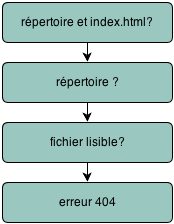
\includegraphics[height=5cm]{Ressources/figure1.png}
  \caption{Organisation des modules pré-définis}
  \label{fig:1}
\end{figure}

\subsection*{Chargement dynamique de code}

Sous Unix, il est possible de charger dynamiquement (c'est à dire à
l'éxecution) un fichier C qui a déjà été compilé au préalable. Cette
technique va nous permettre d'enrichir le serveur web sans avoir à le
recompiler! Sous GNU/Linux, le chargement dynamique nécessite
l'utilisation de la bibliothèque \texttt{dl} et des fonctions
\texttt{dlopen}, \texttt{dlsym}, ... Ces fonctions ne sont pas
détaillées ici car on peut trouver un exemple d'utilisation complet de
ces fonctions dans la page de manuel \texttt{dlopen(3)}. Attention aux
options de compilation, qui sont spécifiques (mais décrites dans le
manuel).  Par ailleurs, un exemple vous est aussi fourni dans le
fichier \texttt{simple-module.c} dans le répertoire
\texttt{ext}\footnote{Ce répertoire contient les modules d'extension
  qui peuvent être chargés dynamiquement. Les module dynamiques
  compilés sont suffixés par \texttt{.so}.}.

\subsection*{Modules supplémentaires}

Les quatre modules de la figure 1 sont pré-définis, et il
correspondent aux modules classiques d'un serveur web. Polyweb,
propose d'autres modules dont les fonctions sont brièvement décrites
ici:
\begin{itemize}
\item \texttt{cgi.so}: ce module permet d'implementer la \textbf{Common
    Gateway Interface}, généralement abrégée
  \href{http://fr.wikipedia.org/wiki/Common\_Gateway\_Interface}{CGI}.

\item \texttt{mytraceuri.so}: ce module permet d'afficher une trace
  pour chaque URI demandée au serveur.

\item \texttt{prettify.so}: ce module permet d'embellir un fichier
  lorsqu'il est chargé par un navigateur Web. Cela peut servir pour
  \emph{"fontifier"} des programmes ou afficher en HTML des fichiers
  \href{http://fr.wikipedia.org/wiki/Markdown}{Markdown}.

\item \texttt{ssi.so}: Ce module permet d'implémenter une version
  simplifiée du mécanisme de
  \href{http://fr.wikipedia.org/wiki/Server_Side_Includes}{Server Side Includes}.
\end{itemize}

Une documentation complète de ces modules est accessible dans
\texttt{doc/doc-extensions.html}

\subsection*{Fichier de configuration}

Lorsque Polyweb démarre, il cherche un fichier de configurations qui
permet de décrire le comportement du serveur. Par défaut, ce fichier
s'appelle \texttt{polywebrc} et il est cherché dans le répertoire courant
(mais il peut aussi être passé en paramètre). Pour ce projet, le plus
simple est de se placer dans le répertoire \texttt{src} pour lancer le
serveur, puisque la configuration se fait de façon relative par
rapport à ce répertoire. Le fichier de configuration permet de spécifier:
\begin{itemize}
\item le répertoire racine du serveur
\item le port sur lequel le serveur tourne 
\item les types MIME reconnus
\item le répertoire où se trouvent les extensions
\item les extensions à charger (attention l'ordre est important: le
  dernier module chargé sera le premier à être exécuté).
\end{itemize}
Un exemple commenté de fichier de configuration est présent dans le
répertoire \texttt{src}. 

\subsection*{Déroulement du projet}

Ce sujet et les fichiers qui l'accompagnent, doivent être considérés
comme une {\bf spécification}, c'est-à-dire que votre programme doit
implémenter exactement ce qui demandé (en particulier l'ajout
inconsidéré de fonctionnalités sera sanctionné). A titre d'exemple et
pour fixer les idées, voici le nombre de lignes sources pour les
parties qui ne vous sont pas livrées:

\begin{verbatim}
  145 ext/cgi.c
   27 ext/mytraceuri.c
   91 ext/prettify.c
  145 ext/ssi.c
  105 src/config.c
  245 src/handler.c
  160 src/http.c
   71 src/mimetype.c
  125 src/misc.c
\end{verbatim}
soit moins de 1150 lignes (commentées). Il n'y a a pas de raison pour
que vous ayez des choses fondamentalement différentes. Si c'est
beaucoup plus gros, c'est que vous vous y êtes probablement mal
pris. N'essayez pas bien sûr de concentrer votre code, au risque de le
rendre illisible, pour tenir dans ces chiffres.

L'évaluation de votre travail prendra en compte principalement la
qualité (et non pas la quantité) du code que vous nous rendrez.

\subsection*{Un module original}

Le travail principal de ce projet consiste à réécrire les fichiers
\texttt{.c} donnés plus haut. Comme cela laisse peu de place à la
créativité, vous devrez aussi implémenter \textbf{un} module personnel
original que vous présenterez au moment de votre soutenance. Pour ceux
qui manquent d'idées, voici une liste de suggestions, que vous pourrez
adapter:
\begin{itemize}
\item un module d'affichage d'images qui renvoie une image retaillée
  si celle-ci est trop grosse
\item un module qui utilise des expression régulières pour changer à la volée le
  texte contenu dans un fichier avnat de l'afficher. Par exemple, remplacer les chaînes
  ``Linux'' par ``GNU/Linux'' pour les puristes.
\item Un module qui fabrique des fichiers de \emph{log} du genre de
  ceux du serveur
  \href{http://en.wikipedia.org/wiki/Common_Log_Format}{Apache}
\item Un module qui ajoute systématiquement un \texttt{?markdown} au
  fichiers suffixés par \texttt{.md} et \texttt{?fontify} aux fichiers
  C, C++, Java, Python, ...
\item ...
\end{itemize}

Soyez inventifs.



\end{document}


% LocalWords:  handler l'URL implémente
